\section{Diskussion}
\label{sec:Diskussion}

% TODO: Sagen, warum bei roter Linie keine Aufspaltung pi-Linie erwartet
% S=0 für beide Zustände, damit normaler Zeeman-effekt
Die rote Linie der Cd-Lampe entsteht durch den Übergang
$^1\mathrm{P}_1 \leftrightarrow ^1\mathrm{D}_2$,
welcher in Abbildung \ref{fig:termschema-rot} dargestellt ist.

\begin{figure}
	\centering
	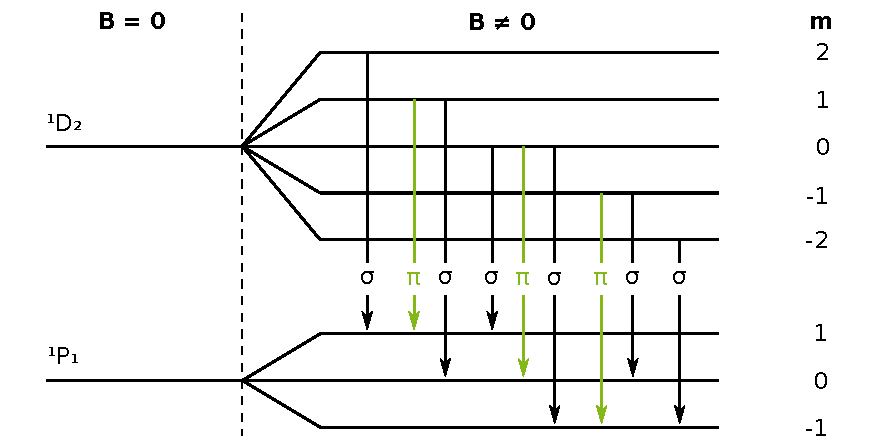
\includegraphics{images/termschema-rot.pdf}
	\caption{Termschema für die rote Linie der \ce{Cd}-Lampe.}
	\label{fig:termschema-rot}
\end{figure}

\begin{figure}
	\centering
	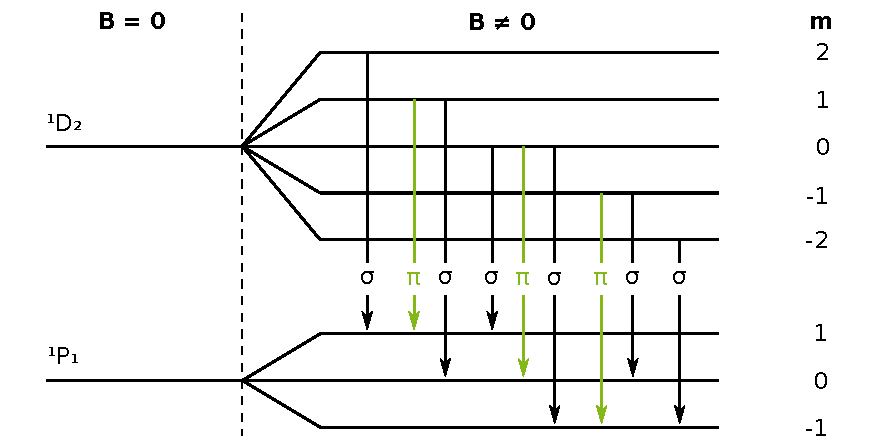
\includegraphics{images/termschema-blau.pdf}
	\caption{Termschema für die blaue Linie der \ce{Cd}-Lampe.}
	\label{fig:termschema-blau}
\end{figure}

- Sagen, dass Pi-Linie bei 10,5 A eingelesen, da hier deutlich höhere Intensität
- Warum nicht alle Peaks eingelesen? -> Zu großes Rauschen, oder nicht bestimmbar

- Systematischer Fehler durch Eichung. Hallsonde musste durchgängig festgehalten werden,
dazu keine Garantie ob immer an selber Position. Magnetfeld jedoch stark ortsabhängig.
Versuch, möglichst nahe an Position der Cd-Lampe heran zu kommen (konnte jedoch nicht heraus genommen werden)
- Bei Stromstärken ~19A kurzschluss, sodass effektiv nur Felder bis ~18A nutzbar.

- Viel mit Justage
- Geringe Intensität der roten Linien durch nicht so intensiven Lichtstrahl
- Bruchstelle an Prisma, sodass ungewollte Reflexe entstehen können (geringere Intensität)
